\title{Лекция 6\\Представление в базе знаний отношений и их свойств}   
\author[]{Шункевич Д.В.}
\institute[]{Белорусский государственный университет информатики и радиоэлектроники}

\begin{frame}
	\titlepage
\end{frame}

\begin{frame}{\\Содержание лекции}
	\topline
	\justifying
	Бинарное отношение и способы его задания. Рефлексивное и антирефлексивное бинарное отношение. Симметричное и антисимметричное бинарное отношение. Транзитивное бинарное отношение. Отношения строгого и нестрогого порядка. Отношения полного (линейного) и частичного порядка. Отношения эквивалентности и толерантности. Квазибинарное отношение. n-арное отношение, схема отношения. Область определения отношения, домен. Операции над отношениями (проекция, соединение, композиция). Метаотношения, примеры. Представление в базе знаний.
\end{frame}

\begin{frame}{\\Понятие отношений}
	\topline
	\justifying
	
	Под \textbf{\textit{отношением}} понимается подмножество декартовой степени множества.\\
	
	\textbf{\textit{Отношение}}, \textit{заданное на множестве М} -- это подмножество \textit{декартового произведения} этого множества самого на себя некоторое количество раз.\\
	
	\scnheader{отношение}
	\scnrelfrom{изображение}{
		\begin{center}
			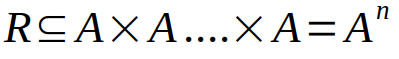
\includegraphics[width=35mm]{figures/sd_sets/relative.png}
			
		\end{center}
	}	
	
	В более широком смысле {\textbf{\textit{отношение}}} -- это математическая структура, которая формально определяет свойства различных объектов и их взаимосвязи.
\end{frame}

\begin{frame}{\\Задание отношений}
	
	
	
	\topline
	\justifying
	
	В теории отношений используются следующие основные типы представления бинарных отношений.\\
	
	\begin{textitemize}
		\item \textit{Путем перечисления элементов}. Отношение R между элементами множеств A и B задается перечислением пар, которые принадлежат R.
		
		\item
		\textit{Матричное представление}. Бинарное отношение представляется в виде \textit{булевой} (двоичной) матрицы.
		
		\item \textit{Графическое представление}. В графическом виде бинарное отношение представляется направленным двудольным графом.
		
	\end{textitemize}
	
\end{frame}

\begin{frame}{\\Классификация отношений}
	
	\topline
	\justifying
	\footnotesize
	
	\begin{SCn}
		\scnheader{отношение}
		
		\begin{scnrelfromset}{разбиение}
			\scnitem{класс равномощных связок}
			\scnitem{класс связок разной мощности}
		\end{scnrelfromset}
		
		\begin{scnrelfromset}{разбиение}
			\scnitem{бинарное отношение}
			\scnitem{небинарное отношение}
		\end{scnrelfromset}
		
		\begin{scnrelfromset}{разбиение}
			\scnitem{ориентированное отношение}
			\scnitem{неориентированное отношение}
		\end{scnrelfromset}
		
		\begin{scnrelfromset}{разбиение}
			\scnitem{ролевое отношение}
			\scnitem{неролевое отношение}
		\end{scnrelfromset}
		
	\end{SCn}
\vspace{-2em}
\end{frame}

\begin{frame}{\\Класс равномощных связок}
	
	\topline
	\justifying	
	
	\begin{SCn}
		\scnheader{класс равномощных связок}
		\scnidtf{класс связок фиксированной арности}
		\scnidtf{отношение, обладающее свойством арности}
		\scnsuperset{унарное отношение}
		\scnsuperset{бинарное отношение}
		\scnsuperset{тернарное отношение}
		\scntext{определение}{\textbf{\textit{класс равномощных связок}} -- это класс связок, имеющих одинаковую мощность.}
	\end{SCn}

\end{frame}	 

\begin{frame}{\\Класс связок разной мощности}
	
	\topline
	\justifying	
	
	\begin{SCn}
		\scnheader{класс связок разной мощности}
		\scnidtf{отношение нефиксированной арности}
		\scnsubset{небинарное отношение}
		\scntext{определение}{\textbf{\textit{класс связок разной мощности}} -- это класс связок, имеющих разную мощность.}
	\end{SCn}
\end{frame}	

\begin{frame}{\\Унарное отношение}%унарное отношение
	\topline
	\justifying
	\begin{SCn}
		\scnheader{унарное отношение}
		\scnidtf{отношение арности один}
		\scnidtf{одноместное множество}
		\scnidtf{множество синглетонов}
		\scntext{определение}{\textbf{\textit{унарное отношение}} -- это множество таких отношений на множестве М, являющихся любым подмножеством множества М.}
	\end{SCn}
\end{frame}

\begin{frame}{\\Бинарное отношение}%бинарное отношение+разбиение
	\topline
	\justifying
	\begin{SCn}
		\scnheader{бинарное отношение}
		\scnidtf{отношение арности два}
		\scnidtf{двухместное отношение}
		\scnsuperset{квазибинарное отношение}
		\scnsuperset{отношение порядка}
		\scnsuperset{отношение толерантности}
		\begin{scnrelfromset}{разбиение}
			\scnitem{рефлексивное отношение}
			\scnitem{антирефлексивное отношение}
			\scnitem{частично рефлексивное отношение}
		\end{scnrelfromset}
		\begin{scnrelfromset}{разбиение}
			\scnitem{симметричное отношение}
			\scnitem{антисемметричное отношение}
			\scnitem{частично симметричное отношение}
		\end{scnrelfromset}
	\end{SCn}
\vspace{-2em}
\end{frame}

\begin{frame}%разбиение бинарного отношения+определение
	\begin{SCn}		
		\scnheader{бинарное отношение}
		\begin{scnrelfromset}{разбиение}
			\scnitem{транзитивное отношение}
			\scnitem{антитранзитивное отношение}
			\scnitem{частично транзитивное отношение}
		\end{scnrelfromset}
		\begin{scnrelfromset}{разбиение}
			\scnitem{ролевое отношение}
			\scnitem{неролевое отношение}
		\end{scnrelfromset}
	\end{SCn}
\scntext{определение}{\textbf{\textit{бинарное отношение}} -- это множество таких отношений на множестве \textbf{\textit{М}}, являющихся подмножеством \textit{ декартова произведения} множества \textbf{\textit{М}}.\\
	Если \textbf{\textit{бинарное отношение R}} задано на \textit{множестве \textbf{M}} и два элемента этого множества \textbf{\textit{a}} и \textbf{\textit{b}} связаны данным отношением, то будем обозначать такую связь как \textbf{\textit{aRb}}.}
\end{frame}

\begin{frame}{\\Квазибинарное отношение}%квазибинарное отношение
	
	\topline
	\justifying
	
	\scnheader{квазибинарное отношение}
	\scntext{пояснение}{ \textbf{\textit{квазибинарное отношение}} -- множество ориентированных пар, хотя бы одним из компонентов которых является связка.\\
		Таким образом, \textit{sc-дуги}, принадлежащие \textbf{\textit{квазибинарным отношениям}}, всегда выходят из связок либо входят в связку.}
	\scnhaselement{разбиение*}
	\scnhaselement{пересечение*}
	\scnhaselement{объединение*}
	
\vspace{-2em}
\end{frame}

\begin{frame}{\\Небинарное отношение}%небинарное отношение
	\topline
	\justifying
	\scnheader{небинарное отношение}
	\scntext{пояснение}{\textbf{\textit{небинарное отношение}} -- это множество отношений, хотя бы одна из связок каждого из которых имеет значение мощности больше двух.}
	\end{frame}

\begin{frame}{\\Ориентированность отношений}%ориентированное и неориентированное отношение
	\topline
	\justifying
	\scnheader{ориентированное отношение}
	\scntext{определение}{\textbf{\textit{ориентированное отношение}} -- это множество таких отношений, каждая связка которых является кортежем.}
	\scnheader{неориентированное отношение}
	\scntext{определение}{\textbf{\textit{неориентированное отношение}} -- это множество таких отношений, каждая связка которых является неориентированным множеством.}
	\end{frame}
	


\begin{frame}{\\Свойства бинарных отношений}
	\topline
	\justifying
	\footnotesize
	\vspace{10mm}
	
	\scnheader{рефлексивное отношение}
	\scntext{определение}{\textbf{\textit{рефлексивное отношение}} на \textit{множестве {\textbf{А}}} -- это \textit{бинарное отношение}, в котором все элементы множества \textbf{\textit{А}} находятся в отношении \textbf{\textit{R}} к самому себе.}
	\scnhaselement{равенство*}
		
	\scnheader{антирефлексивное отношение}
	\scntext{определение}{\textbf{\textit{антирефлексивное отношение R}} на \textit{множестве {\textbf{А}}} -- это \textit{бинарное отношение}, в котором все элементы множества \textbf{\textit{А}} не находятся в отношении \textbf{\textit{R}} к самому себе.}
	\scnhaselement{больше*}
	\scnhaselement{выше*}
	
	\scnheader{частично рефлексивное отношение}
	\scntext{определение}{\textbf{\textit{частично рефлексивное отношение R}} на \textit{множестве {\textbf{А}}} -- это \textit{бинарное отношение}, в котором хотя бы один (но не все) элемент множества \textbf{\textit{А}} находятся в отношении \textbf{\textit{R}} к самому себе.} 
	\end{frame}

\begin{frame}{\\Свойства бинарных отношений}
	\topline
	\justifying
	\scriptsize
	\vspace{10mm}

	\justifying
	\scnheader{симметричное отношение}
	\scntext{определение}{\textbf{\textit{симметричное отношение R}} на \textit{множестве {\textbf{А}}} -- это \textit{бинарное отношение}, в котором для каждой пары элементов \textbf{\textit{a}} и \textbf{\textit{b}} этого множества выполнение отношений \textbf{\textit{aRb}} влечёт выполнение \textbf{\textit{bRa}}.}
	\scnhaselement{параллельность*}
	\scnhaselement{перпендикулярность*}
	\scnhaselement{родственник*}
	
	\scnheader{антисимметричное отношение}
	\scntext{определение}{\textbf{\textit{антисимметричное отношение R}} на \textit{множестве {\textbf{А}}} -- это \textit{бинарное отношение}, в котором для каждой пары элементов \textbf{\textit{a}} и \textbf{\textit{b}} этого множества выполнение отношений \textbf{\textit{aRb}} и \textbf{\textit{bRa}} влечёт равенство \textbf{\textit{a}} и \textbf{\textit{b}}.}
	\scnhaselement{больше*}
	\scnhaselement{выше*}
	
	\scnheader{частично симметричное отношение}
	\scntext{определение}{\textbf{\textit{частично симметричное отношение R}} на \textit{множестве {\textbf{А}}} -- это \textit{бинарное отношение}, в котором для каждой пары элементов \textbf{\textit{a}} и \textbf{\textit{b}} (но не для всех таких пар) этого множества выполнение отношений \textbf{\textit{aRb}} влечёт выполнение \textbf{\textit{bRa}}.}
	\end{frame}

\begin{frame}{\\Свойства бинарных отношений}
	\topline
	\justifying
	\scriptsize
	\vspace{10mm}

	\justifying
	\scnheader{транзитивное отношение}
	\scntext{определение}{\textbf{\textit{транзитивное отношение R}} на \textit{множестве {\textbf{А}}} -- это \textit{бинарное отношение}, в котором для любых трёх элементов этого множества \textbf{\textit{a}}, \textbf{\textit{b}}, \textbf{\textit{c}}выполнение отношений \textbf{\textit{aRb}} влечёт выполнение \textbf{\textit{bRc}} не влечёт выполнение отношения \textbf{\textit{aRc}}.}
	\scnhaselement{параллельность*}
	\scnhaselement{родственник*}

	\scnheader{антитранзитивное отношение}
	\scntext{определение}{\textbf{\textit{антитранзитивное отношение R}} на \textit{множестве {\textbf{А}}} -- это \textit{бинарное отношение}, в котором для любых трёх элементов этого множества \textbf{\textit{a}}, \textbf{\textit{b}}, \textbf{\textit{c}} выполнение отношений \textbf{\textit{aRb}} и \textbf{\textit{bRc}} влечёт выполнение отношения \textbf{\textit{aRc}}.}
	\scnhaselement{перпендикулярность*}
	
	\scnheader{частично транзитивное отношение}
	\scntext{определение}{\textbf{\textit{частично транзитивное отношение R}} на \textit{множестве {\textbf{А}}} -- это \textit{бинарное отношение}, в котором для каждых трех элементов этого множества \textbf{\textit{a}}, \textbf{\textit{b}}, \textbf{\textit{c}} (но не для всех таких троек) выполнение отношений \textbf{\textit{aRb}} влечёт выполнение \textbf{\textit{bRc}} влечёт выполнение отношения \textbf{\textit{aRc}}.}
	
\end{frame}

\begin{frame}{\\Отношение порядка}%отношение порядка 
	\topline
	\justifying
	\begin{SCn}
		\scnheader{отношение порядка}
		\begin{scnrelfromset}{разбиение}
			\scnitem{отношение строгого порядка}
			\scnitem{отношение нестрогого порядка}
			\end{scnrelfromset}
		\begin{scnrelfromset}{разбиение}
			\scnitem{отношение полного порядка}
			\scnitem{отношение частичного порядка}
			\end{scnrelfromset}
		\end{SCn}
	\scntext{определение}{\textbf{\textit{отношение порядка}} -- это \textit{бинарное отношение}, обладающее свойством транзитивности и антисиммитричности.}
\end{frame}
	
\begin{frame}{\\Отношение строгого и нестрого порядка}%отношение строгого и нестрогого 	
\topline
\justifying
	\scnheader{отношение строгого порядка}
	\scntext{определение}{\textbf{\textit{отношение строгого порядка}} -- это \textit{отношение порядка}, обладающее свойством антирефлексивности.}
	\scnhaselement{больше*}
	
	\scnheader{отношение нестрогого порядка}
	\scntext{определение}{\textbf{\textit{отношение нестрогого порядка}} -- это \textit{отношение порядка}, обладающее свойством рефлексивности.}
	\scnhaselement{больше или равно*}
	
	\end{frame}

\begin{frame}{\\Отношение толерантности}%отношение толерантности
	\topline
	\justifying
	\scnheader{отношение толерантности}
	\scntext{определение}{\textbf{\textit{отношение толерантности}} -- это \textit{бинарное отношение}, принадлежащее классам \textit{симметричное отношение} и \textit{рефлексивное отношение}.}
	\end{frame}

\begin{frame}{\\Отношение эквивалентности}%отношение эквивалентности
	\topline
	\justifying
	\begin{SCn}
		\scnheader{отношение эквивалентности}
		\scnidtf{максимальное семейство отношений эквивалентности}
		\scnsubset{отношение толерантности}
		\scnhaselement{равенство*}
		\scntext{определение}{\textbf{\textit{отношение эквивалентности}} -- это \textit{отношение толерантности}, принадлежащее классу \textit{транзитивных отношений}}
		\scntext{примечание}{Каждое отношение эквивалентности уточняет то, что мы считаем эквивалентными сущностями, т.е то, на какие сходства этих сущностей мы обращаем внимание и какие их отличия мы игнорируем (не учитываем).}	
	\end{SCn}
\end{frame}

\begin{frame}{\\Ролевое отношение}%ролевое отношение
	\topline
	\justifying
	\begin{SCn}
		\scnheader{ролевое отношение}
		\scnidtf{атрибут}
		\scnidtf{атрибутивное отношение}
		\scnidtf{отношение, которое задаёт роль элементов в рамках некоторого множества}
		\scnidtf{отношение, являющееся подмножеством отношения принадлежности}
		\scnrelto{семейство подмножеств}{принадлежность*}
		\scnsubset{бинарное отношение}
		\scnsuperset{числовой атрибут}

		\scntext{пояснение}{\textbf{\textit{ролевое отношение}} -- это отношение, являющееся подмножеством отношения принадлежности.}
	\end{SCn}
\end{frame}

\begin{frame}%ролевое отношение пример
	\scntext{правило идентификации экземпляров}{В конце каждого \textit{идентификатора}, соответствующего экземпляра класса \textbf{\textit{ролевое отношение}}, не являющегося системным, ставится знак " \scnrolesign ".
		
		Например:\\
		\textit{ключевой экземпляр\scnrolesign}
		
		Из-за ограничений в разрешенном алфавите символов, в системном идентификаторе не может быть использовать знак ``\scnrolesign'', поэтому в начале каждого \textit{системного идентификатора}, соответствующего экземплярам класса \textbf{\textit{ролевое отношение}} ставится префикс ``rrel\_''.
		
		Например:\\
		\textit{rrel\_key\_sc\_element}}
	\end{frame}
	
\begin{frame}{\\Числовой атрибут}%числовой атрибут
    \topline
    \justifying

	\begin{SCn}
	\scnheader{числовой атрибут}
	\scnidtf{порядковый номер}
	\scnidtf{номер компонента ориентированной связки}
	\scnhaselement{\textbf{1\scnrolesign}; \textbf{2\scnrolesign}; \textbf{3\scnrolesign}; \textbf{4\scnrolesign}; \textbf{5\scnrolesign}; \textbf{6\scnrolesign}; \textbf{7\scnrolesign}; \textbf{8\scnrolesign}; \textbf{9\scnrolesign}; \textbf{10\scnrolesign}}; ...
	\scntext{пояснение}{\textbf{\textit{числовой атрибут}} -- \textit{ролевое отношение}, задающее порядковый номер элемента некоторой ориентированной связки, не уточняя при этом семантику такой принадлежности. Во многих случаях бывает достаточно использовать числовые атрибуты, чтобы различать компоненты связки, семантика каждого из которых дополнительно оговаривается, например, при определении отношения, которому данная связка принадлежит.}
	\end{SCn}
\end{frame}	
	
\begin{frame}{\\Неролевое отношение}%неролевое отношение
	\topline
	\justifying
	\begin{SCn}
		\scnheader{неролевое отношение}
		\begin{scnrelfromset}{разбиение}
		\scnitem{небинарное отношение}
		\scnitem{неролевое бинарное отношение}
		\end{scnrelfromset}
		\scntext{пояснение}{\textbf{\textit{неролевое отношение}} -- отношение, не являющееся подмножеством отношения принадлежности.}
		\end{SCn}
	\end{frame}

\begin{frame}%неролевое отношение пример
	
		\scntext{правило идентификации экземпляров}{В конце каждого \textit{идентификатора}, соответствующего экземплярам класса \textbf{\textit{неролевое отношение}}, не являющегося системным, ставится знак ``*''.
			
			Например:\\
			\textit{включение*}
			
			Из-за ограничений в разрешенном алфавите символов, в системном идентификаторе не может быть использовать знак ``*'', поэтому в начале каждого \textit{системного идентификатора}, соответствующего экземплярам класса \textbf{\textit{неролевое отношение}} ставится префикс ``nrel\_''.
			
			Например:\\
			\textit{nrel\_inclusion}}
		\end{frame}

\begin{frame}{\\Неролевое бинарное отношение}%неролевое бинарное отношение	
    \topline
    \justifying	
   	\begin{SCn}
		\scnheader{неролевое бинарное отношение}
		\scntext{пояснение}{\textbf{\textit{неролевое бинарное отношение}} -- \textit{бинарное отношение}, не являющееся \textit{ролевым отношением}.}
	\end{SCn}
\end{frame}

\begin{frame}{\\Арность}%арность
	\topline
	\justifying
	\begin{SCn}
		\scnheader{арность}
		\scnidtf{арность отношения}
		\scniselement{параметр}
		\scntext{пояснение}{\textbf{\textit{арность}} -- это параметр, каждый элемент которого представляет собой класс \textit{отношений}, каждая связка которых имеет одинаковую \textit{мощность}. Значение данного \textit{параметра} совпадает со значением \textit{мощности} каждой из таких связок.}
	\end{SCn}
\end{frame}

\begin{frame}%арность пример
	\begin{SCn}		
	\scnrelfrom{описание примера}{
		\begin{center}
		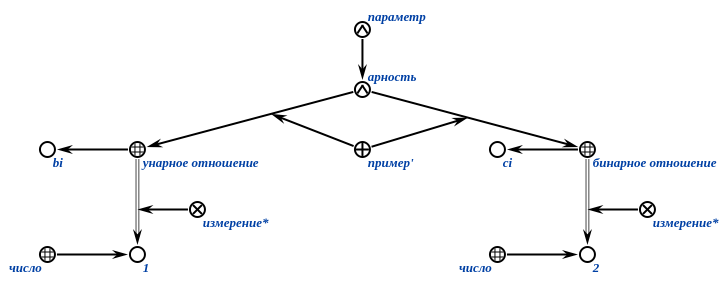
\includegraphics[width=120mm]{figures/sd_sets/arity.png}
	\end{center}}
\end{SCn}
\end{frame}
	
\begin{frame}{\\Область определения}%область определения
	\topline
	\justifying
	\begin{SCn}
		\scnheader{область определения*}
		\scnidtf{область определения отношения*}		
		\scniselement{бинарное отношение}
		\scntext{пояснение}{\textbf{\textit{область определения*}} -- это \textit{бинарное отношение}, связывающее отношение со множеством, являющимся его областью определения.
			
		Областью определения отношения будем называть результат теоре\-ти\-ко-мно\-жественного объединения всех связок этого отношения, или, другими словами, результат теоретико-множественного объединения всех множеств, являющихся доменами данного отношения.}
	\end{SCn}

\end{frame}

\begin{frame}%область определения пример		
		\begin{SCn}
		\scnrelfrom{описание примера}{
			\begin{center}
			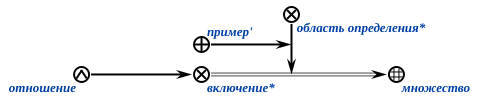
\includegraphics[width=100mm]{figures/sd_sets/domain.png}
		\end{center}}
	\end{SCn}
\end{frame}

\begin{frame}{\\Атрибут отношения}%атрибут отношения		
	\topline
	\justifying
	\begin{SCn}
	\scnheader{атрибут отношения*}
	\scnidtf{ролевой атрибут, используемый в связках заданного отношения*}
	\scniselement{бинарное отношение}
	\scntext{пояснение}{\textbf{\textit{атрибут отношения*}} -- это \textit{бинарное отношение}, связывающее заданное отношение с \textit{ролевым отношением}, используемым в данном отношении для уточнения роли того или иного элемента связок данного отношения.}
	\end{SCn}
\end{frame}

\begin{frame}%атрибут отношения пример		
		\scnrelfrom{описание примера}{
			\begin{center}
			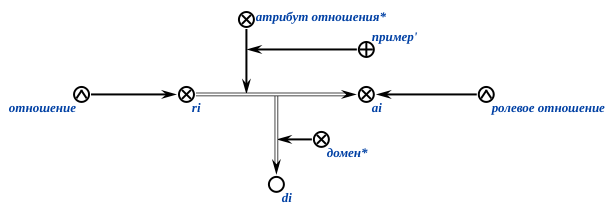
\includegraphics[width=120mm]{figures/sd_sets/relationshipAttribute.png}
		\end{center}}
	\end{frame}
	
\begin{frame}{\\Домен}%домен
	\topline
	\justifying
	\begin{SCn}
	\scnheader{домен*}
	\scnidtf{домен отношения по заданному атрибуту*}
	\scniselement{бинарное отношение}
	\scntext{пояснение}{\textbf{\textit{домен}} -- это \textit{бинарное отношение}, связывающее связку отношения \textit{атрибут отношения*} со множеством, являющимся доменом заданного отношения по заданному атрибуту. Множество \textbf{\textit{di}} является доменом отношения \textbf{\textit{ri}} по атрибуту \textbf{\textit{ai}} в том и только том случае, если элементами этого множества являются все те и только те элементы связок отношения \textbf{\textit{ri}}, которые имеют в рамках этих связок атрибут \textbf{\textit{ai}}.}
	\end{SCn}
\end{frame}

\begin{frame}%домен приер	
	\scnrelfrom{описание примера}{
		\begin{center}
		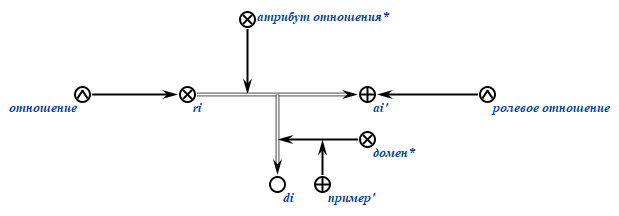
\includegraphics[width=120mm]{figures/sd_sets/domen.png}
	\end{center}}
\end{frame}

\begin{frame}{\\Первый домен}%первый домен
\topline
\justifying
	\begin{SCn}
	\scnheader{первый домен*}
	\scniselement{бинарное отношение}
	
	\scntext{определение}{\textbf{\textit{первый домен*}} -- это \textit{бинарное отношение}, связывающее отношение с множеством, являющимся доменом по атрибуту \textbf{\textit {1\scnrolesign}} данного отношения.}
	\scnrelfrom{описание примера}{
		\begin{center}
		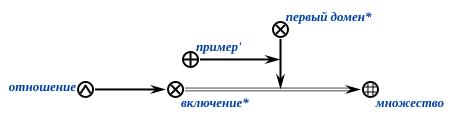
\includegraphics{figures/sd_sets/firstDomen.png}
	\end{center}}
	\end{SCn}
\end{frame}

\begin{frame}{\\Второй домен}%второй домен
	\topline
	\justifying
	\begin{SCn}
	\scnheader{второй домен*}
	\scniselement{бинарное отношение}
	\scntext{определение}{\textbf{\textit{второй домен*}} -- это \textit{бинарное отношение}, связывающее отношение с множеством, являющимся доменом по атрибуту \textbf{\textit{2\scnrolesign}} данного отношения.}
	\scnrelfrom{описание примера}{
		\begin{center}
		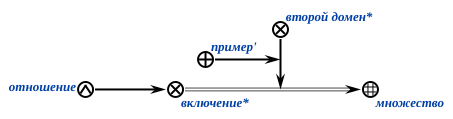
\includegraphics{figures/sd_sets/secondDomen.png}
	\end{center}}
	\end{SCn}
\end{frame}
	
\begin{frame}{\\Композиция отношений}%композиция отношений
	\topline
	\justifying
	\begin{SCn}
	\scnheader{композиция отношений*}
	\scniselement{квазибинарное отношение}

	\scntext{определение}{\textbf{\textit{композиция отношений*}} -- это \textit{квазибинарное отношение}, связывающее два бинарных отношения с отношением, являющимся их композицией. Под композицией бинарных отношений \textbf{\textit{R}} и \textbf{\textit{S}} будем понимать множество $\{(x, y) | \exists z(xSz \wedge zRy)\}$}
	\end{SCn}
\end{frame}

\begin{frame}%композиция отношений пример
	\scnrelfrom{описание примера}{
		\begin{center}
		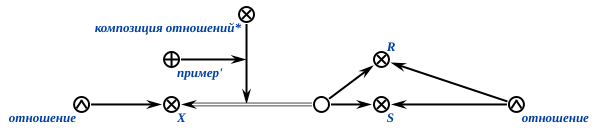
\includegraphics[width=120mm]{figures/sd_sets/relationshipComposition.png}
	\end{center}}
	\end{frame}
	
\begin{frame}{\\Фактор-множество}%фактор-множество
	\topline
	\justifying
	\begin{SCn}
		\scnheader{фактор-множество*}
		\scnidtf{быть фактор-множеством*}
		\scnidtf{множество всевозможных максимальных множеств из попарно эквивалентных элементов*}
		\scnidtf{множество всевозможных классов эквивалентности для заданного отношения эквивалентности*}
		\scniselement{бинарное отношение}

		\scntext{определение}{\textbf{\textit{фактор множество*}} -- это бинарное ориентированное отношение, каждая связка которого связывает некоторое отношение эквивалентности со множеством всех соответствующих этому отношению классов эквивалентности. Каждый такой класс представляет собой максимальное множество сущностей, каждая пара которых принадлежит указанному выше отношению эквивалентности.}
	\end{SCn}
\end{frame}

\begin{frame}%фактор-множества пример		
	\scnrelfrom{описание примера}{
	\begin{center}
		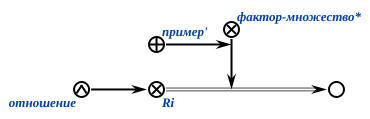
\includegraphics[width=80mm]{figures/sd_sets/factor_set.png}
	\end{center}}
\end{frame}

\begin{frame}{\\Метаотношение}%метаотношение
	\topline
	\justifying
	\begin{SCn}
		\scnheader{метаотношение}
		\scntext{определение}{метаотношение -- это \textit{отношение}, в каждой связке которого есть по крайней мере один компонент, являющийся знаком некоторого \textit{отношения}.}
		\scnhaselement{домен*}
		\scnhaselement{атрибут отношения*}
		\scnhaselement{область определения*}
	\end{SCn}
\end{frame}



	


